% Torus, Klein bottle and projective plane as glued polygons.
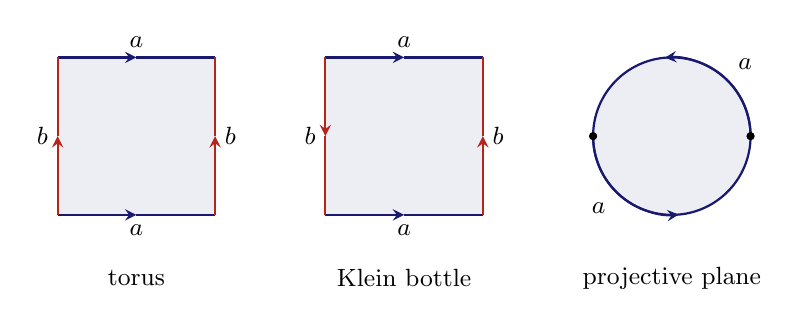
\begin{tikzpicture}[font=\small,>=stealth,x=1cm,y=1cm]
\tikzset{e/.style={thick,MidnightBlue},f/.style={thick,BrickRed}}
% torus a b a^{-1} b^{-1}
\begin{scope}
\fill[MidnightBlue!8] (0,0) rectangle (2,2);
\draw[e,->] (0,0) -- (1,0); \draw[e] (1,0) -- (2,0); \node[below] at (1,0) {$a$};
\draw[e,->] (0,2) -- (1,2); \draw[e] (1,2) -- (2,2); \node[above] at (1,2) {$a$};
\draw[f,->] (2,0) -- (2,1); \draw[f] (2,1) -- (2,2); \node[right] at (2,1) {$b$};
\draw[f,->] (0,0) -- (0,1); \draw[f] (0,1) -- (0,2); \node[left] at (0,1) {$b$};
\node at (1,-0.8) {torus};
\end{scope}
% Klein bottle a b a^{-1} b
\begin{scope}[xshift=3.4cm]
\fill[MidnightBlue!8] (0,0) rectangle (2,2);
\draw[e,->] (0,0) -- (1,0); \draw[e] (1,0) -- (2,0); \node[below] at (1,0) {$a$};
\draw[e,->] (0,2) -- (1,2); \draw[e] (1,2) -- (2,2); \node[above] at (1,2) {$a$};
\draw[f,->] (2,0) -- (2,1); \draw[f] (2,1) -- (2,2); \node[right] at (2,1) {$b$};
\draw[f,->] (0,2) -- (0,1); \draw[f] (0,1) -- (0,0); \node[left] at (0,1) {$b$};
\node at (1,-0.8) {Klein bottle};
\end{scope}
% projective plane: disc with boundary aa
\begin{scope}[xshift=7.8cm,yshift=1cm]
\fill[MidnightBlue!8] (0,0) circle (1);
\draw[e] (0,0) circle (1);
\draw[e,->] (1,0) arc (0:95:1); \draw[e,->] (-1,0) arc (180:275:1);
\fill (1,0) circle (1.5pt); \fill (-1,0) circle (1.5pt);
\node[above right] at (0.72,0.72) {$a$}; \node[below left] at (-0.72,-0.72) {$a$};
\node at (0,-1.8) {projective plane};
\end{scope}
\end{tikzpicture}
